\subsection{Software Architecture Requirements}

Figure \ref{fig_design} illustrates the generic Software Architecture of the Artifacts.
Each element instantiation will comply to the Element Naming Convention laid out int
appendix \ref{appendix_element_naming_convention}. In the subsequent table we will layout
the requirements specific for each of the elements.

\begin{figure}[H]
    \centering
    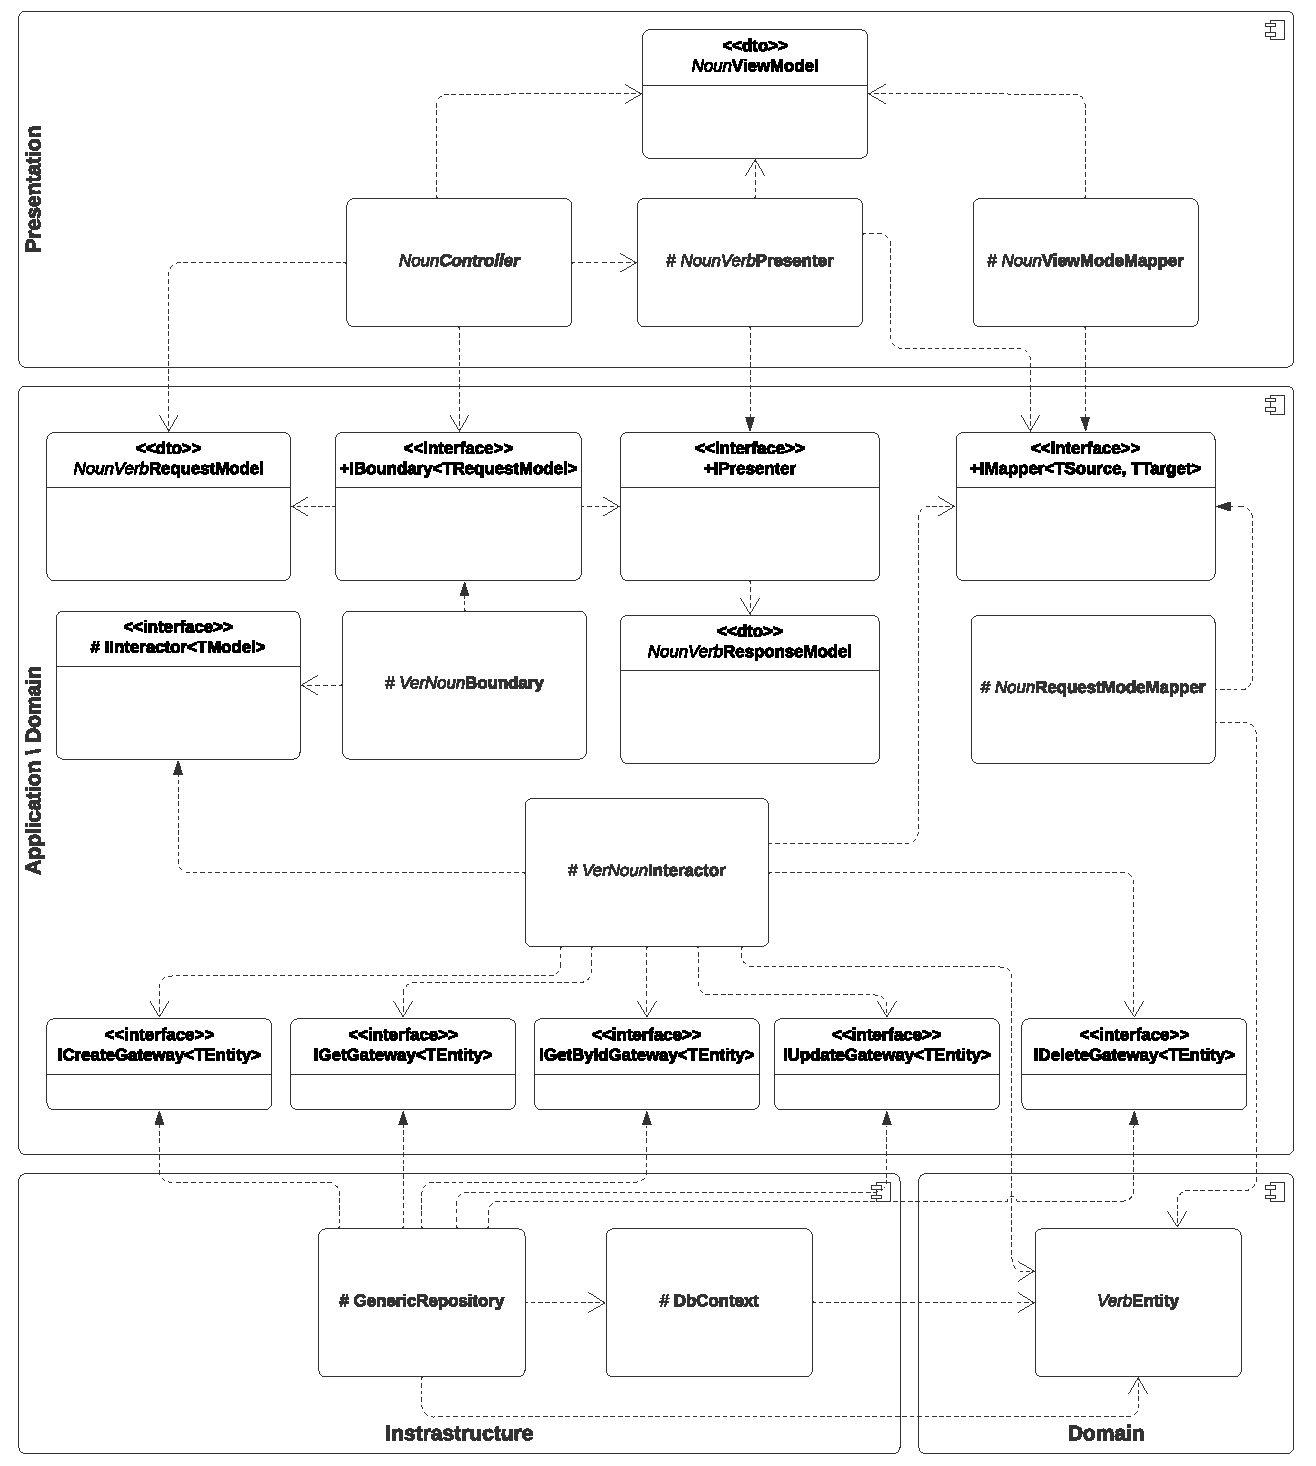
\includegraphics[width=1\textwidth]{figures/generic_design.pdf}
    \caption[Generic architecture]{The Generic architecture of the artifacts}
    \label{fig_design}
\end{figure}

% \begin{tabular}{ \makebox[3em][r]{\rownumber\space}} p{0.87\linewidth} }
%     \multicolumn{1}{@{\makebox[3em][r]{Nr.}} | r}{\emph{Requirement}}\\ 

\subsubsection*{Presentation Layer elements}
\begin{table}[H]
    \begin{tabular}{@{\makebox[2em][c]{\rownumber\space}}  p{0.87\linewidth}}
        \multicolumn{1}{@{\makebox[2em][c]{Nr.}}  p{0.87\linewidth}}{Requirement}\\ 
    \hline
       The ViewModel will mainly contain fields representing data attributes of the
       corresponding Entity. Additionally, The ViewModel can contain information specific
       the the (user)interface. \\

       The ViewModel will have no èxternal dependencies to other objects part of the
       Architecture. \\
       
       \hline
    \end{tabular}
\caption{ViewModel Requirements}
\label{table_requirements_viewmodel}
\end{table}

\begin{table}[H]
    \begin{tabular}{@{\makebox[2em][c]{\rownumber\space}}  p{0.87\linewidth}}
        \multicolumn{1}{@{\makebox[2em][c]{Nr.}}  p{0.87\linewidth}}{Requirement}\\ 
    \hline
    The Presenter Implementation is a derivative of the IPresenter interface,
    locatedin the Applciation Layer. \\   
    
    When applicable, the Presenter will map the ResponseModel to the ViewModel using the IMapper
    interface \\
    
    When applicable, the Presenter is responsible for preparing the HTTP Response.\\
    The Presenter will have an internal visibility.\\
    
    \hline
    \end{tabular}
\caption{Presenter Requirements}
\label{table_requirements_presenter}
\end{table}

\begin{table}[H]
    \begin{tabular}{ m{0.05\linewidth} p{0.87\linewidth} }
    \hline
    \textbf{Nr.} & \textbf{Description} \\ 
    \hline
       1. & When applicable, the Presenter will map the ResponseModel to the ViewModel using the IMapper
       interface \\
       2. & When applicable, the Presenter is responsible for preparing the HTTP Response.\\
       3. & The Presenter will have an internal visibility.\\
       \hline
    \end{tabular}
\caption{ViewModelMapper Requirements}
\label{table_requirements_viewModelMapper}
\end{table}